 \subsection{PRISM}
 PRISM is a probabilistic model checker that allows formal modelling and analysis of systems that exhibit random or probabilistic behaviour. In our case, we will use PRISM to model a Continuous-Time Markov Chain (CTMCs) but there are other models that can be be modeled thanks to this tool. \\
 With Uppaal we were able to assert that there were no conflicting state and that our system is safe. Thanks to PRISM, we will be able to show that our is system if fair. Every traffic lights will get the green light in a fair way, meaning that there will be no starvation for one of them. Moreover, thanks to PRISM, we can show the statistics of green light times for every different actor, something that is not possible to do in Uppaal.
 
\begin{figure}[h]\label{fig:prism}
  \begin{center}
    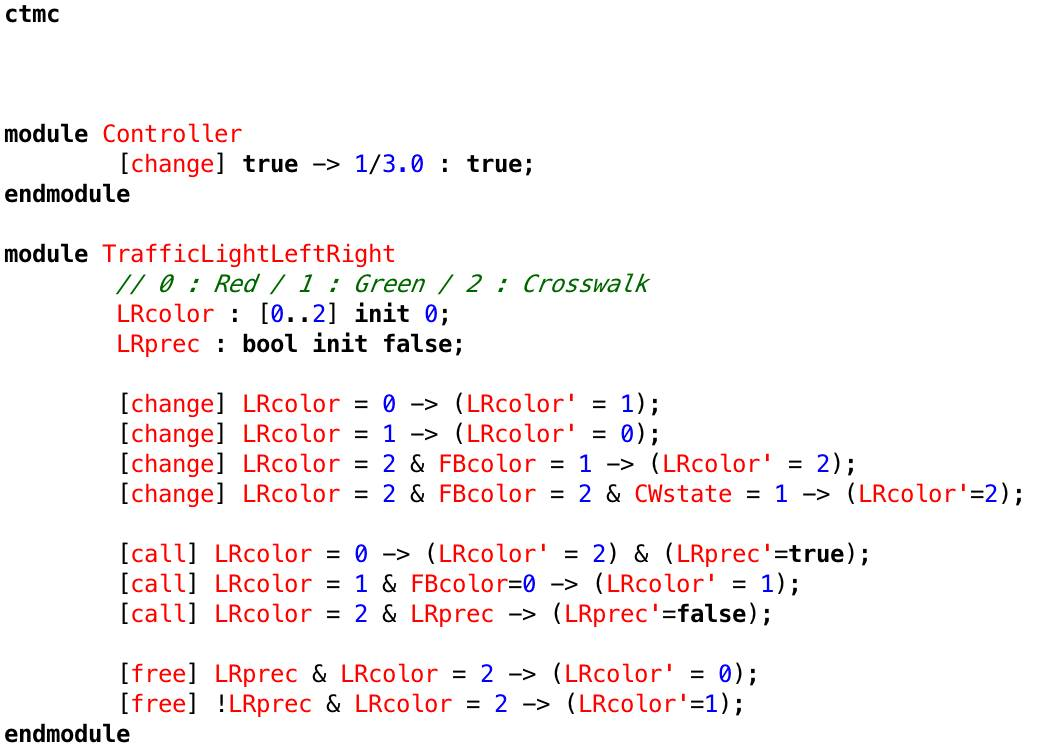
\includegraphics[width=0.8\textwidth]{picture/prism.png}
    \caption{Example of the PRISM language}
  \end{center}
\end{figure} 


